\documentclass[article]{report}             % Type of document

\usepackage[utf8]{inputenc}    		 	    % Encoding
\usepackage[english]{babel}			        % Language
\usepackage{geometry}           			% Page margin
\usepackage{graphicx}           			% For images
\usepackage{newcent}            			% Font
\usepackage{color}              			% Colors
\usepackage{listings}           			% Lists
\usepackage[footnote, nolist]{acronym}	    % Acronyms
\usepackage[absolute, overlay]{textpos}	    % Text positioning
\usepackage[babel=true]{csquotes}

\usepackage{fancyhdr}          			 % We might have a need for them
\usepackage{float}
\usepackage{tabularx}

\usepackage{latexsym}
\usepackage{pdfpages}
\usepackage{tikz}
\usepackage{ifthen}
\usepackage{wrapfig}
\usepackage{textcomp}
\usepackage{multicol}

\usepackage{listings} % includes code

\lstset{
	tabsize=4,
	language=matlab,
        basicstyle=\scriptsize,
        %upquote=true,
        aboveskip={0.5\baselineskip},
        columns=fixed,
        showstringspaces=false,
        extendedchars=true,
        breaklines=true,
        basicstyle=\normalsize,
        prebreak = \raisebox{2ex}[2ex][2ex]{\ensuremath{\hookleftarrow}},
        showtabs=false,
        showspaces=false,
        showstringspaces=false,
        identifierstyle=\ttfamily,
        keywordstyle=\color[rgb]{0,0,1},
        commentstyle=\color[rgb]{0.133,0.545,0.133},
        stringstyle=\color[rgb]{0.627,0.126,0.941},
	language=Java
}

\setlength{\columnsep}{1cm}
\setlength{\TPHorizModule}{\paperwidth}	% Used for textblock
\setlength{\TPVertModule}{\paperheight}	% Used for textblock

\title {Oral Presentation 1}
\parskip = 0.25cm              % Summary options (spaces between lines)

% Margin
\geometry{tmargin=2.5cm, bmargin=1.5cm, lmargin=2.5cm, rmargin=2cm}

\definecolor{blue}{rgb}{0.13,0.29,0.46}
\definecolor{red}{rgb}{1,0,0}
\definecolor{couleur_titre}{rgb}{0.20, 0.45, 0.80}
\definecolor{couleur_nom}{rgb}{0.11, 0.6, 0.18}

\renewcommand{\labelitemi}{$\bullet$}
\renewcommand{\contentsname}{Table of contents}

% Title at the top of the page
\pagestyle{fancyplain} \chead{}\lhead{\textit{Team Dedalus}} \rhead{\textcolor{couleur_titre}{\emph{\textit{Project: SkyLands}}}}

\title {Book of specifications}
\author {Romain\and Renaud\and Aenora\and Erwan}
\date {}

%
% Document
%
\begin{acronym}
	\acro{OO}{Oriented-Object}
	\acro{RTS}{Real Time Strategy}
	\acro{FPS}{First Person Shooter}
	\acro{Mogre}{Managed Object-Oriented Graphics Rendering Engine}
	\acro{API}{Application Progamming Interface}
	\acro{GUI}{Graphical User Interface}
	\acro{MyGUI}{Multilayer and overlappable GUI System}
	\acro{IDE}{Integrated Developement Environment}
	\acro{AI}{Artificial Intelligence}
	\acro{NPC}{Non Player Character}
	\acro{UML}{Unified Modeling Language}
	\acro{PHP}{PHP : Hypertext Preprocessor}
	\acro{ORM}{Object-Relational Mapping}
	\acro{MVC}{Model View Controller}
	\acro{OGRE}{Object-Oriented Graphics Rendering Engine}
\end{acronym}
\begin{document}
	\thispagestyle{empty}
  	\begin{titlepage} 
		\vspace*{1cm} 
  		\begin{center} 
  			{\huge{\textsc{1st Oral} \\ ~ \\{\large From}\\ ~\\ Team \\  ~ \\ }}
	  		\includegraphics[width = 14cm]{images/Titles/Dedalus.png}
			\\ ~ \\ ~ \\ ~ \\ ~ \\ ~ \\ ~ \\ ~ \\ ~ \\ ~ \\ ~ \\ ~ \\ ~ \\ ~ \\ ~ 
		\end{center}
  		\hfill {\large Romain \textsc{Biessy}}
  		\hfill {\large Renaud \textsc{Gaubert}}
  		\hfill {\large Aenora \textsc{Tye}}
  		\hfill {\large Erwan  \textsc{Vasseure}}
  	\end{titlepage} 

  	\tableofcontents
  		\pagenumbering{arabic}
  		\newpage
		
		\chapter{\textcolor{blue}{Introduction}}
 			It has been two month since the last presentation. Two month is a short time and we had a lot to do the task was almost daunting. Indeed, when we learned that we did not have all points on the progress, not only did we want to realize all the task written in the book of specifications but we had to do more. \\

 			And more, meant to us, impressing terrain generation, amazing FPS through a complete rewritting of the displaying system an even better GUI than planned, a console and awesome physics such as Jumping all around the place. \\

 			However, creating those features were really time consuming, we literally spent days coding them and, throughout this report we will show you the best of our game.
  		\chapter{\textcolor{blue}{Communications}}
			\section{Twitter, Facebook and YouTube }
				Since our game is starting to be playable, we wanted to show the world what it looked like.\\
				To do so, we created accounts on the two main social networking web sites: Facebook and Twitter. Also to give people the possibility to really have an idea of what our game look like, we have made a small footage showing the main goal of our game and it's advancement and posted it on Youtube.

				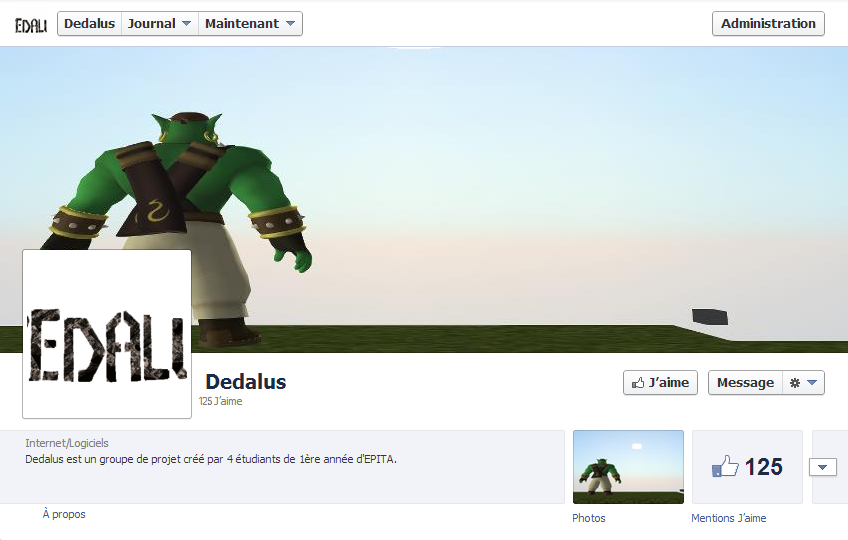
\includegraphics[width = 17cm]{images/Graphics/fb.png}
				\newpage

			\section{Web site}
				You might have seen it at the first oral presentation, our website was a little bit empty. Knowing that we made some efforts, and added some pages to the website. The first we added was the download page, the second we added was the page World. Finally, we created an admin area where we could edit the news on the front page.

				This is done using an SQL database, this means as we are using Symfony, we use Doctrine. An example of Doctrine is the following class (this is not all the class) : 
\begin{lstlisting}
<?php
/* @ORM\Table()
 * @ORM\Entity(repositoryClass="SkyLands\KernelBundle\Entity\NewsRepository") */
class News {
    /**
     * @var integer
     * @ORM\Column(name="id", type="integer")
     * @ORM\Id
     * @ORM\GeneratedValue(strategy="AUTO")
     */
    private $id;

    /**
     * @var string
     * @ORM\Column(name="author", type="string", length=255)
     */
    private $author;
    /**
     * @var string
     * @ORM\Column(name="message", type="text")
     */
    private $message;


    /*Get id
     * @return integer 
     */
    public function getId() { return $this->id; }}
?>
\end{lstlisting}
\newpage
 		Thanks to symfony, creating the file and launching a php command line Symfony will detect all new doctrine class (marked with a @ORM comment) and update the database for us (creating a table).\\
 		Also creating a new row in a table and reading from a table is made easier with doctrine : 
\begin{lstlisting}
<?php
//writting
$article = new News();
$article->setTitle('2nd Oral presentation');
$article->setAuteur('Dedalus');

$em = $this->getDoctrine()->getManager();
$em->persist($article);
$em->flush();

//reading
$repository = $this->getDoctrine()->getManager()->
getRepository('SkyLandsKernelBundle:News');

$newsList   = $repository->findBy(array(), array('date' => 'desc'), 4, 0);
//newsList is an array of array access it with newsList[i][fieldName]
?>
\end{lstlisting}
		
						

						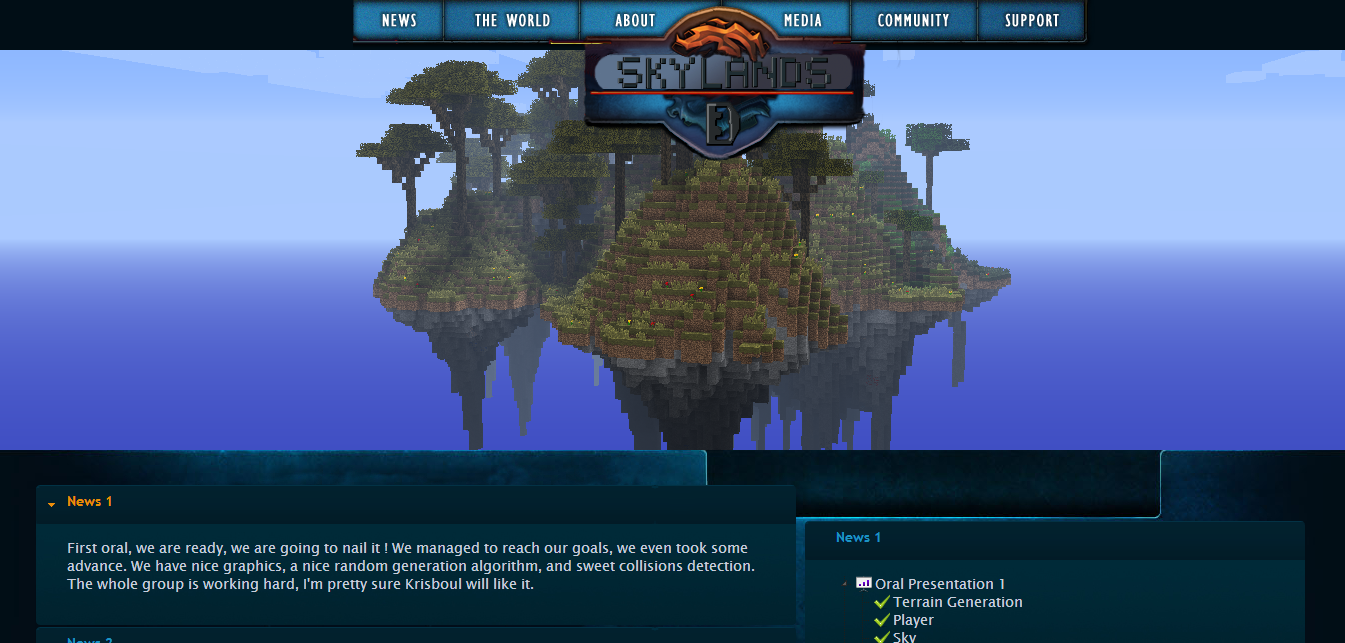
\includegraphics[width=16cm]{images/Graphics/web.png}
					

		\chapter{\textcolor{blue}{Licensing}}
			At Dedalus, we consider that Licensing our code is an important task. According to the French legal code, a license is an authorization.\\
			First, we explored the available licenses and, one of the first license we were directed to was the GNU GPL.

			\section{GNU LGPL}
\begin{textblock}{0.475}(0.120, 0.470)
				
The GNU Lesser General Public License or LGPL (formerly the GNU Library General Public License) is a free software license published by the Free Software Foundation (FSF). \\
The LGPL allows developers and companies to use and integrate LGPL software into their own (even proprietary) software without being required (by the terms of a strong copyleft) to release the source code of their own software-parts. Merely the LGPL software-parts need to be modifiable by end-users (via source code availability): therefore, in the case of proprietary software, the LGPL-parts are usually used in the form of a shared library (e.g. DLL), so that there is a clear separation between the proprietary parts and open source LGPL parts.\\
				\end{textblock}

				\begin{textblock}{0.628}(0.600, 0.495)
					\begin{figure}
						
\includegraphics[width=6.5cm]{images/LGPL.png}
					\end{figure}
				\end{textblock}
~\\~\\~\\~\\~\\~\\~\\~\\~\\~\\~\\~\\~\\
				However one of the downside of the LGPL is that if you do not use the code in a DLL, so you put it in your code, your project automatically gets under the LGPL. It is usually said that the licence is viral. That is one the only thing we do not agree with.

			\section{BSD license}
				BSD licenses are a family of permissive free software licenses, imposing minimal restrictions on the redistribution of covered software. This is in contrast to copyleft licenses, which have reciprocity share-alike requirements. The original BSD license was used for its namesake, the Berkeley Software Distribution (BSD), a Unix-like operating system. The original version has since been revised and its descendants are more properly termed modified BSD licenses.
				This is the license we choose. Basically, anyone can copy our source code choose the license he wants or even choose to make his code proprietary. But he must say that he used our code. This was the only condition we wanted on our source code.\\
Here are the terms of our license : \\

Redistribution and use in source and binary forms, with or without
modification, are permitted provided that the following conditions are met: 

1. Redistributions of source code must retain the above copyright notice, this list of conditions and the following disclaimer. \\
2. Redistributions in binary form must reproduce the above copyright notice, this list of conditions and the following disclaimer in the documentation and/or other materials provided with the distribution.\\

THIS SOFTWARE IS PROVIDED BY THE COPYRIGHT HOLDERS AND CONTRIBUTORS enquote{"AS IS"} AND
ANY EXPRESS OR IMPLIED WARRANTIES, INCLUDING, BUT NOT LIMITED TO, THE IMPLIED
WARRANTIES OF MERCHANTABILITY AND FITNESS FOR A PARTICULAR PURPOSE ARE
DISCLAIMED. IN NO EVENT SHALL THE COPYRIGHT OWNER OR CONTRIBUTORS BE LIABLE FOR
ANY DIRECT, INDIRECT, INCIDENTAL, SPECIAL, EXEMPLARY, OR CONSEQUENTIAL DAMAGES
(INCLUDING, BUT NOT LIMITED TO, PROCUREMENT OF SUBSTITUTE GOODS OR SERVICES;
LOSS OF USE, DATA, OR PROFITS; OR BUSINESS INTERRUPTION) HOWEVER CAUSED AND
ON ANY THEORY OF LIABILITY, WHETHER IN CONTRACT, STRICT LIABILITY, OR TORT
(INCLUDING NEGLIGENCE OR OTHERWISE) ARISING IN ANY WAY OUT OF THE USE OF THIS
SOFTWARE, EVEN IF ADVISED OF THE POSSIBILITY OF SUCH DAMAGE.\\

The views and conclusions contained in the software and documentation are those
of the authors and should not be interpreted as representing official policies, 
either expressed or implied, of the FreeBSD Project.\\

				\begin{textblock}{0.628}(0.325, 0.450)
					\begin{figure}
						
\includegraphics[width=6.5cm]{images/BSD.jpeg}
					\end{figure}
				\end{textblock}
		

		\chapter{\textcolor{blue}{Terrain display}}
			\section{What was done}
				For the 1st oral presentation, the display system was the biggest problem we had, FPS were very low, around 30, even though we only displayed little Islands (5*5*5 chunks, which are 16*16*16 blocks tall).\\

This system consisted in displaying visible faces of each blocks a unique entity. MOGRE had troubles supporting thousands of faces at a time thus limiting the maximum size of an Island.

			\section{Optimizations}
				So we came up with another idea, which was a bit risky. Basically creating an entity in mogre is very simple :\\
\begin{lstlisting}

ManualObject block = new ManualObject("name");
block.Begin("texture here", RenderOperation.OperationTypes.OT_TRIANGLE_LIST);

	block.Position(new Vector3(0,   0,     0));
	block.Position(new Vector3(0,   100,   0));
	block.Position(new Vector3(100, 0,     0));
	block.Position(new Vector3(100, 100,   0));

	block.Quad(0, 1, 2, 3);
block.End();

\end{lstlisting}

As you can see, we only have to give the object position and to tell to draw a quad (which is actually a shortcut to creating 2 triangles).
Basically, the idea we had was to gather all visible blocks of the same material in an instance of an object (which was called multiblock). However this was not simple for 2 reasons :
\begin{itemize}
\item We cannot tell the material to delete a face at a certain position neither can we add new faces to it
\item We wanted blocks which had more than one texture on it (for example the grass cube doesn't have the same texture on the the top face than on the bottom
 face)
 \end {itemize}

First of all you need to understand our architecture : 
				\begin{figure}[h]
					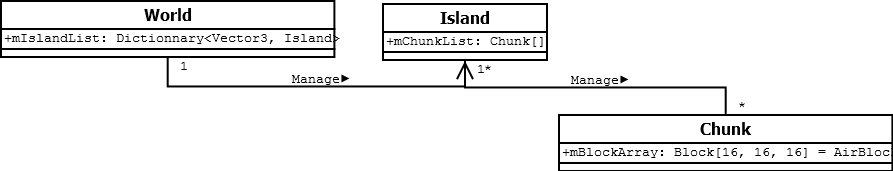
\includegraphics[scale=0.5]{images/Hierarchy.png}
				\end{figure}

As you can see here each chunk contains an array of block. At first, in this array, we stored in each cell a new instance of an object (The cube object) which had an attribute defining it's material.\\

However this way was memory consuming and unadapted for the future uses of the blocks (e.g. GUI). Thus, to save memory we rewrote the this part of the code and now it is more Object oriented and developer friendly : 

				\begin{figure}[h]
				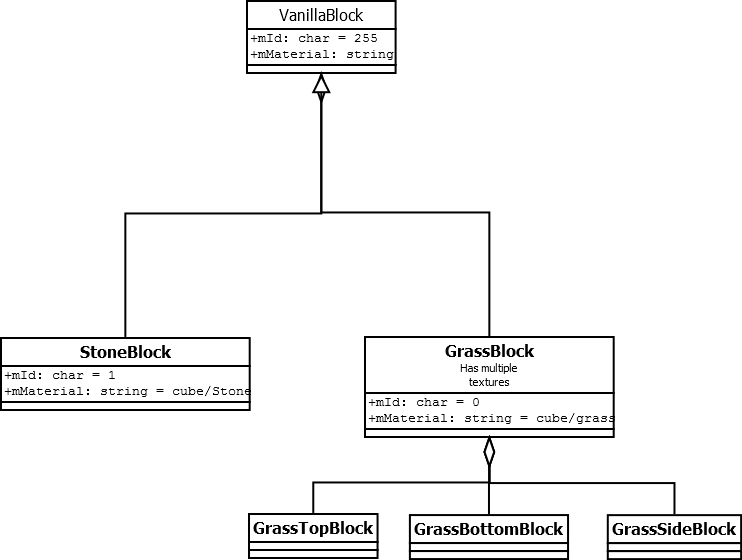
\includegraphics[scale=0.5]{images/cubes.png}
				\end{figure}

Basically, using reflexion, in a static constructor of Chunk, we instantiate an object in charge of displaying each blocks in the namespace containing the blocks except, abstract class, the airBlock and class which has class inheriting from.\\
Thus, in this example, the following blocks would be instantiated : stoneBlock, GrassTopBlock, GrassBottomBlock, GrassSideBlock. Obviously in our code there are way more blocks 
than in this example.\\


This system may seem a bit complicated, and it was, but it was totally worth the cost, we increased the frame rate by 20, and it now turns around 400FPS. Also, the Islands size were trippled, getting from 4*4 to 12*12 (on the x, z coordinates with y the height) and can even be increased to 30 * 30. This means that if we assimilated the terrain as one continuous layer of block we would have : 	30 * 30 * 16 * 16 = 230400 cubes, counting only top faces and bottom faces : 460800 faces and 921600 triangles, around 1 000 000 triangles (with about 100 FPS).
			
			\section{Sky}
				At the first oral, we presented you a sky using the library Caelum but then we wanted to try another well-known library : SkyX. Once again we actually used a wrapper of the original library coded in C++. We wanted to try another library so that we could choose the best for our game.\\
				
Unfortunately it appeared that even if SkyX is a great library in C++ its wrapper is much less interesting. Indeed many functions weren't implemented in the wrapper. This lack leads to a far less awesome render than in the C++ version. Besides we had lots of troubles integrating this library to our project because of the different existing versions of Mogre.\\

That's why we ended up choosing Caelum. But we didn't make this choice because it was the first we saw but because this is the best one we can have. \\

				\includegraphics[width = 16cm]{images/Graphics/sky.png}
		\chapter{\textcolor{blue}{Player actions}}
			\section{Adding blocks}
				Our player can now add blocks on the terrain using the mouse. A cursor at the center of the screen help to see the targeted block. \\

The first difficulty was to compute the actual position of this cursor in the 3 dimensional world. Then we cast a ray in the camera's direction so that we check if there already is a block. Computing the position of the new block is only half of the work, we then had to add the faces at the right position.\\

				One of the downside of gathering all faces in one object is that you can't add faces to the object. Therefore we had to think a bit outside the object. What we did was the following : When the player adds cube to the terrain, we display the face as an independent object. And  we remember the position where he added a block. When he has added 30 blocks, we launch a new thread whose role is to recreate each multiblocks that were modified.\\

				First this thread must change the list of Vector3 of the instance of each multiblock which were modified and add the blocks the player added to it's list. Then he must recreate the object and when it's done remove the old one and replace it with a new one. C\# having a thread system which is easy to handle, this part was pretty easy. \\


				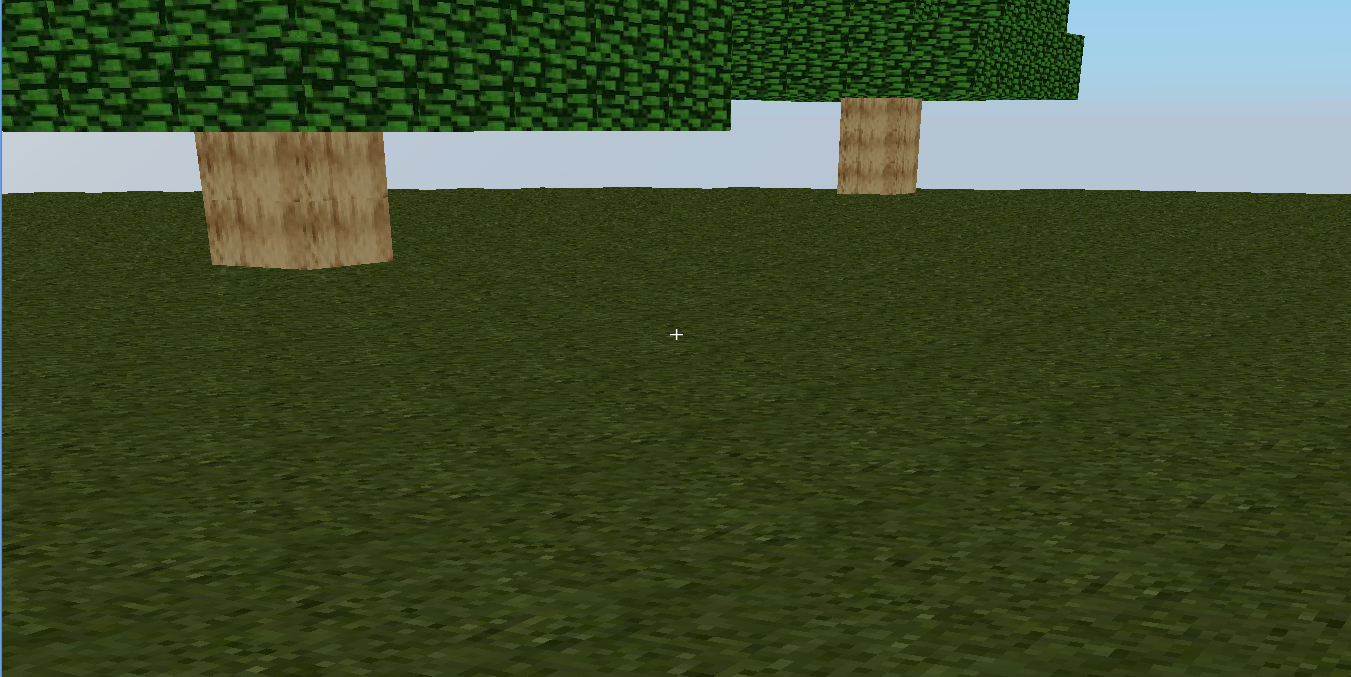
\includegraphics[width = 8cm]{images/Graphics/beforeAdd.png}		
				\includegraphics[width = 8cm]{images/Graphics/afterAdd.png} \newpage

				
				
			\section{Removing Blocks}
				If we can add block this would be great if we could remove blocks as well. So that's what we did. Computing the position of the targeted block the same work as for adding blocks.

				On the other hand removing blocks from the scene was a tricky part. Because the function we needed was not implemented in C\# (traveling through the Manual object and modifying the faces, which are vector3) we had to get it from the C++ libraries. And, what's more, when we found the function we needed, we discovered the function needed pointers, thus so we had to use the unsafe option.\\

				The basic idea is that a Manual Object is just a buffer of pointers to a Vector3 (actually it's a pointer to an array of size 3 which represent the coordinates of the vector3). Thus we had to get the vertex buffer, Lock it, get the position of the first element and from there on tell what was the face number we wanted to access, and multiply this number by the \enquote{size} of a Vector3 this would set the pointer to the right position. From there on we only had to set for a face, it's 4 coords to 0 and check how many faces were visible.\\

				However 2 problems arose : the first block with multiple textures, had to be dealt with in a separate way. \\
				The second was that when removing a block, we had to refresh the surrounding blocks, thus most of the time creating faces which were not in the manual object, that was the cause of a bug where we tried to suppress faces which were not in the manual object. You can imagine that it was deleting other faces than the one we wanted deleted.\\

				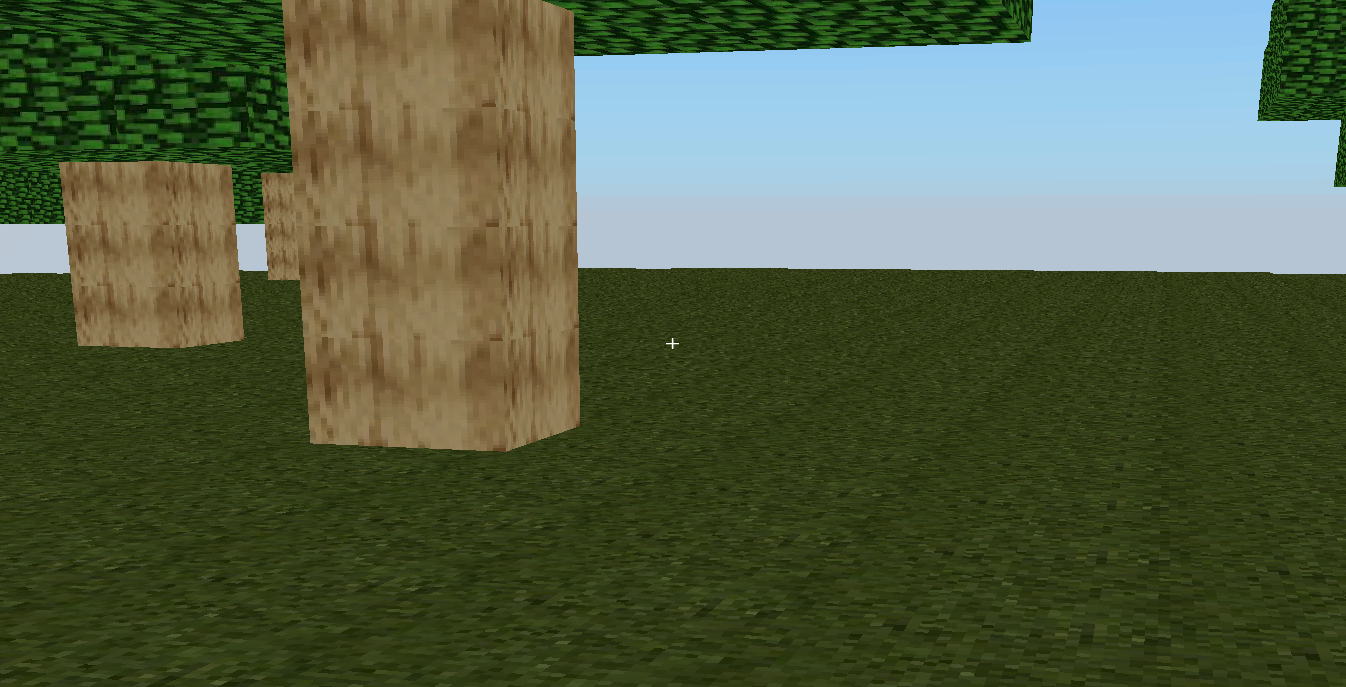
\includegraphics[width = 8cm]{images/Graphics/before.png}		
				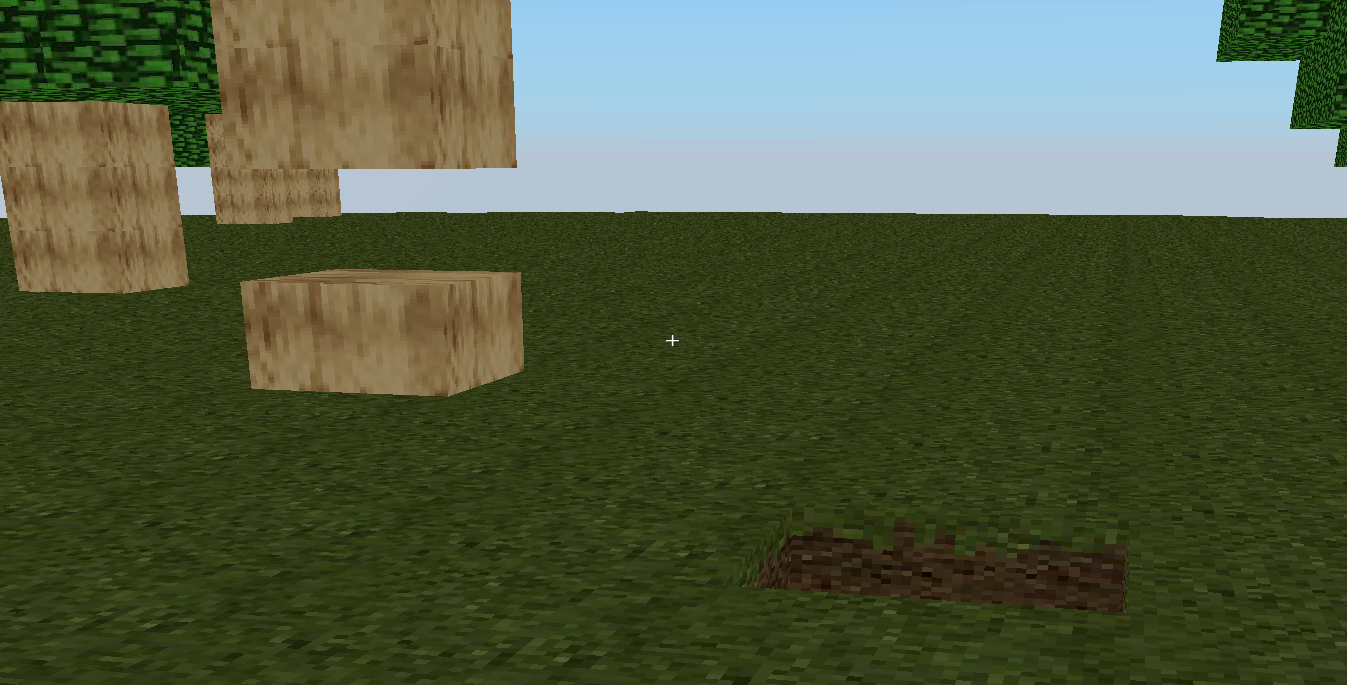
\includegraphics[width = 8cm]{images/Graphics/after.png} \\



		\chapter{\textcolor{blue}{Terrain generation}}
			\section{A new structure}
				After the first oral, we wished for a more modable, and more object oriented structure. Thus most of the code was rewritten, allowing us to first create island which were not using Perlin 3D and secondly, when generating the terrain have what we called \enquote{populators} which were called after the terrain was generated.\\

				Thus, in game you will now see trees and cactus as well. We can also set what we call the \enquote{ground cover} which define which blocks you'll find on the first second and third layer of the ground. 
				
			\section{Perlin 3D algorithm}
				Thanks to our display optimization, we can now generate bigger islands. On the other hand the terrain's generation algorithm is still an algorithm of complexity O(n) (we have to travel through the terrain in the 3 dimensions). And can not be as optimized as the display.\\



				Our Perlin 3D algorithm still works combining 3d noise in a polynomial expression :

				\begin{lstlisting}

double noiseValue = (noise[xx, yy, zz]) * noise2[xx, 255 - yy, zz] + noise[xx, yy, zz] - System.Math.Abs(1 / smoothHeight * (yy - smoothHeight - minElevation + 20))

				\end{lstlisting} 
~\\

				Basically, perlin noise generate solid terrain and not islands. Removing the absolute value of 1/elevation to the noise value ensure that we get a more Island shaped terrain.\\
				The 2nd degree polynomial and the smoothHeight + 20 is a form we came after hours of testing. \\

				Combining a bigger terrain and and an upgraded perlin algorithm gave us nice results : 
				
				\begin{figure}[h]
					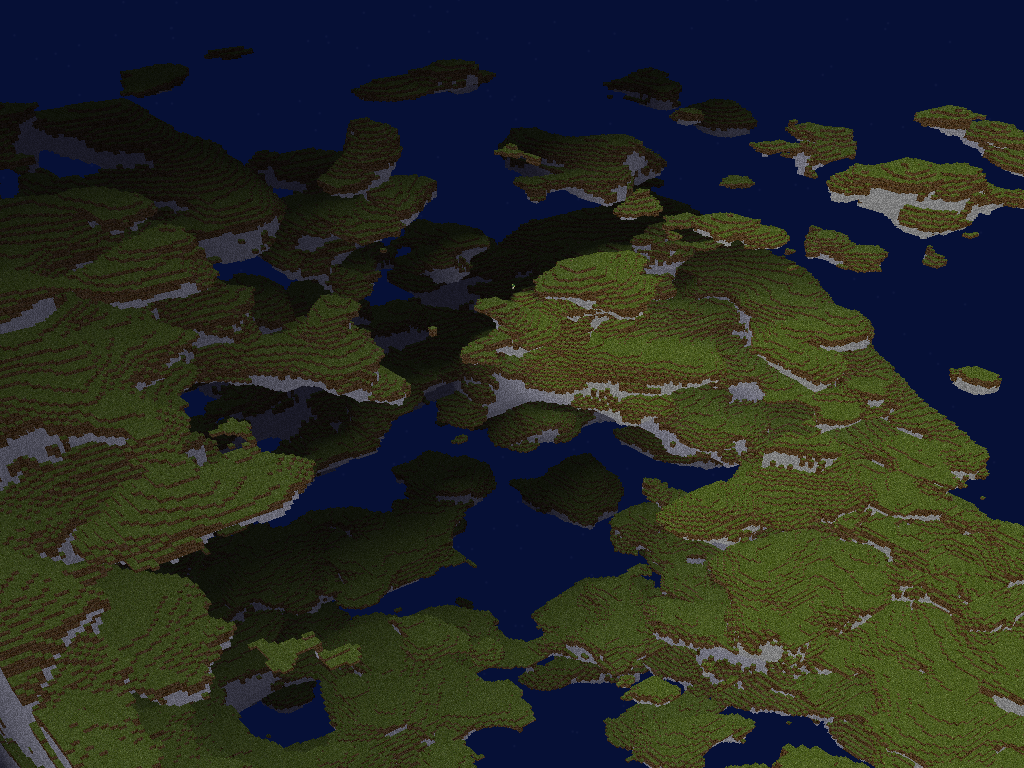
\includegraphics[scale=0.25]{images/terrain01.png}
					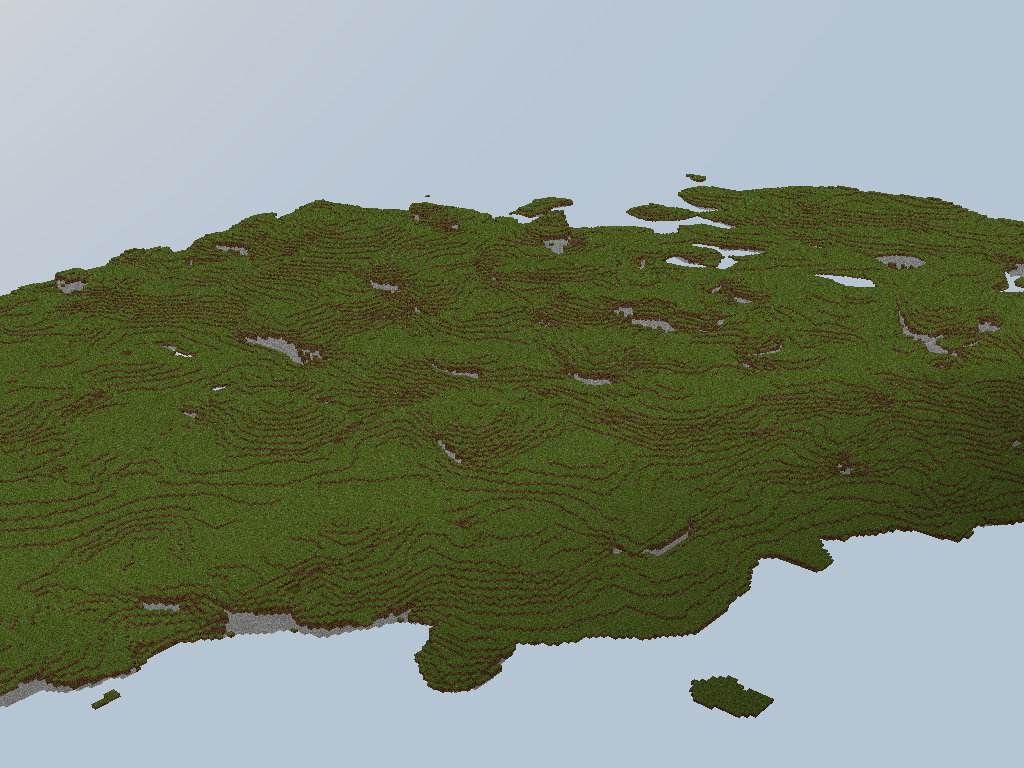
\includegraphics[scale=0.25]{images/terrain02.png}
				\end{figure}

				~\\~\\ ~\\
			\section{Biomes}
				You must have noticed in the previous formula the minElevation variable. This is an essential part of the terrain generation. When it's low value, the terrain is flatter. Whereas a higher value will generate multiple levels and \enquote{mountains}. \\

				Therefore we took advantage of this and created what we called the class Biome which not only had a value determining the minElevation variable but also had the ability to change the blocks on the ground (ground cover) and had populators.


		\chapter{\textcolor{blue}{Buildings}}
			\section{Constructions blocks}
				Unlike in Minecraft, our player can build some presaved buildings. This is the basic of a Starcraft-like game. These buildings will allow the players to spawn some bots for his army and also to gather few basic resources.\\

We don't want the player to build all of the constructions block per block, all he will have to do is to place a \enquote{construction block}. Then when he clicks this block, a menu opens and the player will have to give the required resources to start the construction. For now we haven't the inventory system with the actual resources of the player that's why the construction menu is light.\\

For this oral presentation, our buildings are simple. The player will actually be able to save his own buildings for the fourth presentation, this is part of the \enquote{map editor}.
			
			\section{Saving and loading the structure and terrain}
				This wasn't very complicated, basically as we already explained you a block has an id which is a char. We only had to save each char in a file using a StreamWritter so as a byte.\\
				This is how it works : foreach Islands, call the function save. This function will create a new file in the users' AppData/Roaming/SkyLands called Islands-Position.\\

				It will write in the file it's X, Y, Z size (in chunks and not in blocks) and then begin to write the information using 3 simple for loops.
				The results talk for themselves, for 100 000 blocks = 100 000 bytes = 100 ko. which would be around the number of blocks contained in a 15 * 15 island.
				
		\chapter{\textcolor{blue}{Physics}}
			\section{Collisions}
				As we want the best of our game, we tried to implement the library MogreNewt. This library provides a physic engine and handle collisions detection. It is a powerful tool but it implies to add each cube one by one as a \enquote{Body} that is to say about 80 000 blocks. This leads to an important loss of FPS which is definitely what we don't want. Here you can see all the wires of the bodies including the character which was automatically created using its mesh file.\\

Eventually, we kept our system using the height points of each corner since we consider our character as a parallelepiped rectangle. This isn't an AABB collision algorithm because we look at the type of block there are next to the points.

			\section{Jump}
				As promised our characters can now jump. Once the collisions with the floor worked this wasn't a hard task. We use a second order polynomial to determine the actual speed of the jump depending on the time since the character has jumped. Then our gravity system takes cares to make him fall.
				
		\chapter{\textcolor{blue}{Character}}

		\chapter{\textcolor{blue}{AI}}
			\section{Pathfinding}
				Pathfinding refers to the plotting, by a computer application, of the shortest route between two points. At its core, a pathfinding algorithm searches a graph by starting at one vertex and exploring adjacent nodes until the destination node is reached. Althought graph searching methods such as a beadth-first search would find a route if given enougth tmie, other methods, which explore the graph, would tend to reach the destination sooner. \\
 It is useful when integrating an IA. With it, a character will dodge holes and dead ends. An example use of the pathfinding : if an enemy see the player, the algorithm will find the shortest path the enemy can take to come and attack the player.
			\section{A star (A*)}
				The A* (A star) is an algoritgm wildely used in pathfinding and graph traversal, the process of plotting an efficently traversable path between points, called nodes. Noted for its performance and accuracy, it enjoys widespread use.\\
 The A* uses a best-first search and finds a least-cost path from a given initial node to one goal node. As A* traverses the graph, it follows a path of the lowest expected total cost or distance, keeping a sorted priority queue of alternate path segments along the way. \\
			\begin{center}
				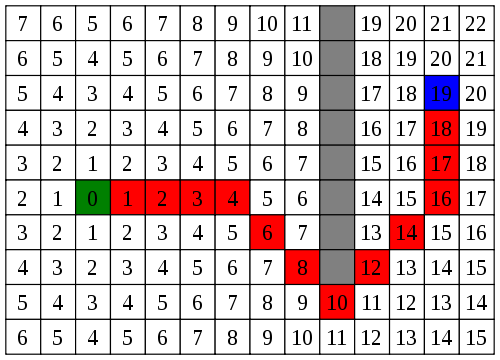
\includegraphics[width = 8cm]{images/Graphics/AStar.png}	
			\end{center}		
\chapter{\textcolor{blue}{Menu}}
			\section{Console}
				Something we understood is that we need a console in game to gather some informations directly. Most 
of the time this is temporary informations but this is still useful.  We used a system of listener so that we 
could be notified anywhere in the code that the player entered a command.  That’s why we can easily for 
instance get the character position.  \\

			\section{New menu}
				Since the last oral presentation, we added many menus.  First, we have some options in the main menu. 
We also added an intermediate menu in game for the escape key and menu when we click on a construction 
block.  \\

				\begin{center}
					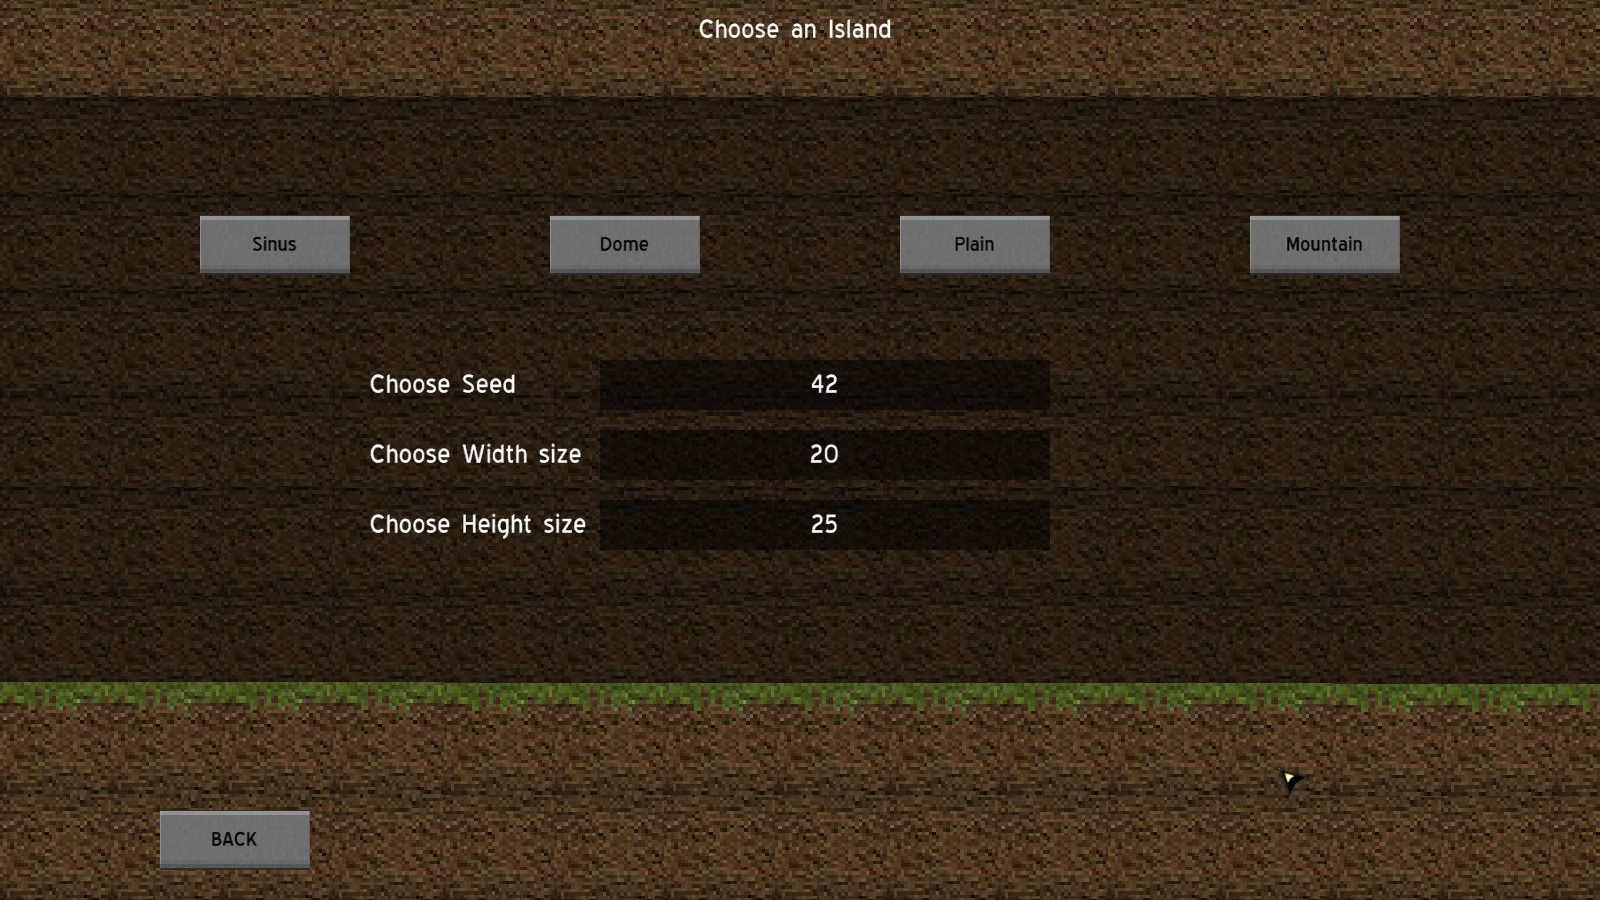
\includegraphics[width = 16cm]{images/Graphics/menuNew.png}	
				\end{center}	


		\chapter{\textcolor{blue}{Conclusion}}

			This is the end of our fabulous report ! We hope you enjoyed it, and that it intresseted you.  We are convinced that the goals of this oral presentation were reached, and that we did more than what was written in ou book of specification (Jump, display optimization, saving and loading the world. \\
		Most of our  work was directed towards the optimization part because of the fact that 25 fps is clearly not enough for what was going to be added (AI and shadows). It would have caused huge lags.\\

Finally, we already have an impressive game and we don't intend to stop now. We intend to finish this game, make it more playable and even more awesome

\end{document}